\subsection{CopyConstPropFold.fs}
The optimization done in 'copyConstPropFold.fs' revolves around substituting longer abstract syntax tree expressions with smaller more optimized abstract syntax tree expressions. For instance, a long expression involving multiplication with zero will always result in zero, and thus as soon we see we are doing multiplication with zero we can just return the optimized expression zero. This optimization along with optimization for multiplication with one has been implemented on lines 85-97 in CopyConstPropFold.fs as seen below.\\
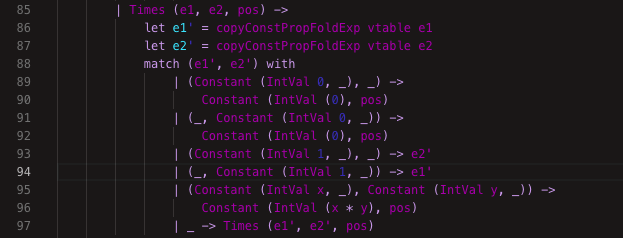
\includegraphics[width=\linewidth]{Materials/Optimization/Times}\\
Similarly short circuiting has been implemented on lines 98-107 for \textit{And}.\\
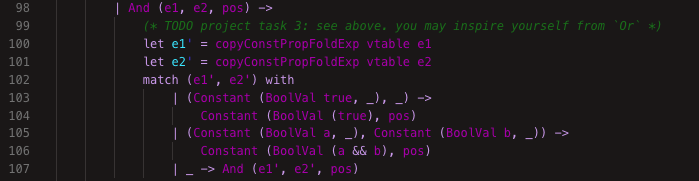
\includegraphics[width=\linewidth]{Materials/Optimization/And}\\
Following the instructions in the lecture slides\footnote{Lecture slides, 9-Optim-Fasto.pdf} the cases for \textit{Var, Index} and \textit{Let bindings} has been implemented. In the case of \textit{Var} we look in the symbol table for the variable, if it exists we replace it with an abstract syntax tree of its value, otherwise we do nothing. For the \textit{Index} case we attempt to optimize the expression and then look up the name of the array in the symbol table. If the name exists we replace the former abstract syntax tree with a new one constructed as the new name and the optimized expression. Otherwise we construct a new 'Index' abstract syntax tree with the old name and the optimized expression (lines 24-45 in CopyConstPropFold.fs).\\
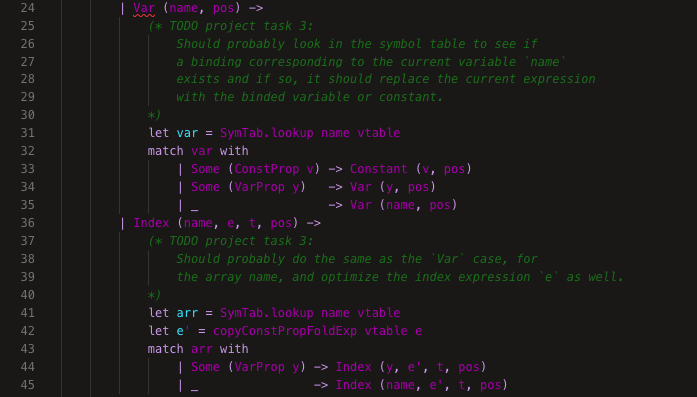
\includegraphics[width=\linewidth]{Materials/Optimization/VarIndex}\\
The last case \textit{Let} can be split into another three cases: \textit{Var, Constant} and \textit{Let}. In all cases the expression is always optimized.\\
In the case of \textit{Var}, a binding of the outer \textit{Let} name is made with the variable and added to the symbol table. The outer \textit{Let} body is then attempted optimized according to this new symbol table. And lastly a new 'Let' abstract syntax tree is constructed with the outer \textit{Let} name, the optimized expression and the optimized outer \textit{Let} body. Similarly is done for \textit{Constant}. If we reach the \textit{Let} case we rearrange the let bindings such that they get optimized and we run \textit{copyConstPropFoldExp} to optimize this new expression. All of this is done on lines 46-81 of CopyConstPropFold.fs.\\
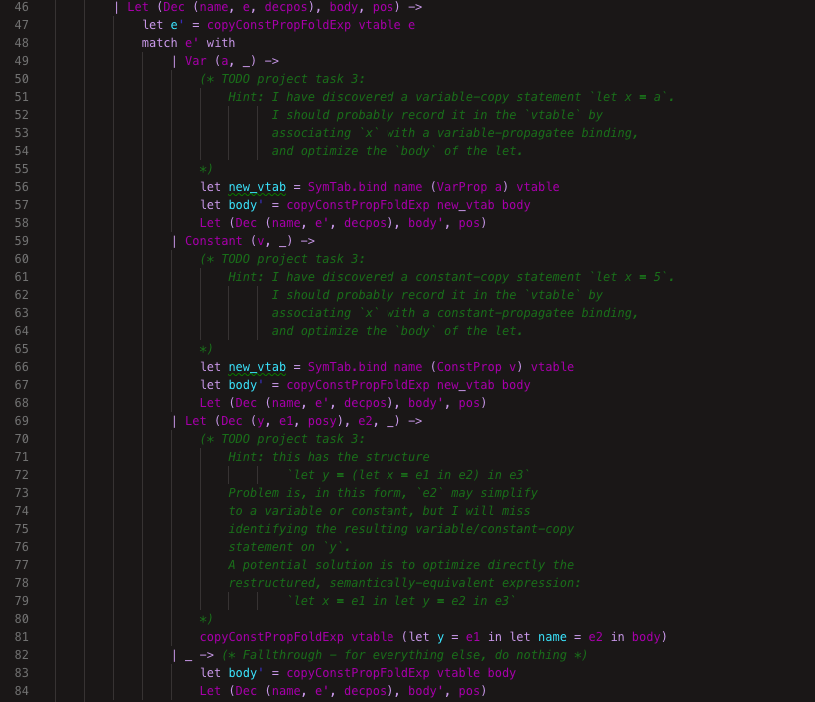
\includegraphics[width=\linewidth]{Materials/Optimization/Let}